\section{АНАЛИЗ ПРЕДМЕТНОЙ ОБЛАСТИ}
\label{sec:analysis}

При проектировании программного продукта, который решает реальные задачи пользователя, очень важно выяснить главный фукционал и свойства продукта, чтобы сервис отвечал запросам пользователей и производство продукта было оправдано.

Требования к ПО определяют, какие свойства и характеристики оно должно иметь для удовлетворения потребностей пользователей и других заинтересованных лиц. Однако сформулировать требования к сложной системе не так легко. В большинстве случаев будущие пользователи могут перечислить набор свойств, который они хотели бы видеть, но никто не даст гарантий, что это — исчерпывающий список. Кроме того, часто сама формулировка этих свойств будет непонятна большинству программистов.

Чтобы ПО было действительно полезным, важно, чтобы оно удовлетворяло реальные потребности людей и организаций, которые часто отличаются от непосредственно выражаемых пользователями желаний. Для выявления этих потребностей, а также для выяснения смысла высказанных требований приходится проводить достаточно большую дополнительную работу, которая называется анализом предметной области или бизнес-моделированием, если речь идет о потребностях коммерческой организации. В результате этой деятельности разработчики должны научиться понимать язык, на котором говорят пользователи и заказчики, выявить цели их деятельности, определить набор задач, решаемых ими. В дополнение стоит выяснить, какие вообще задачи нужно уметь решать для достижения этих целей, выяснить свойства результатов, которые хотелось бы получить, а также определить набор сущностей, с которыми приходится иметь дело при решении этих задач. Кроме того, анализ предметной области позволяет выявить места возможных улучшений и оценить последствия принимаемых решений о реализации тех или иных функций.

После этого можно определять область ответственности будущей программной системы — какие именно из выявленных задач будут ею решаться, при решении каких задач она может оказать существенную помощь и чем именно. Определив эти задачи в рамках общей системы задач и деятельностей пользователей, можно уже более точно сформулировать требования к ПО.

Анализом предметной области занимаются системные аналитики или бизнес-аналитики, которые передают полученные ими знания другим членам проектной команды, сформулировав их на более понятном разработчикам языке. Для передачи этих знаний обычно служит некоторый набор моделей, в виде графических схем и текстовых документов.

Анализ деятельности крупной организации, такой как банк с сетью региональных отделений, нефтеперерабатывающий завод или компания, производящая автомобили, дает огромные объемы информации. Из этой информации надо уметь отбирать существенную, а также уметь находить в ней пробелы — области деятельности, информации по которым недостаточно для четкого представления о решаемых задачах. Значит, всю получаемую информацию надо каким-то образом систематизировать. 

Далее приводится анализ сведений, которые влияют на формулирование требований, выбор архитектуры и дальнейшее проектирование и разработку программного средства.

Для начала нужно понять, какие они — современные сервера. Т.е. следует изучить стек технологий, а также понять, какие параметры и функционал важны для пользователя.    


\subsection{Серверная архитиктура}
\label{sec:analysis:serv_arch}

Соверменная серверная архитектура направлена на улучшения производительности продукта. Сейчас существуют два основные вида архетектуры: микросервисы и монолитные сервера.

«Микросервисы» — еще один новый термин на шумных улицах разработки ПО. И хотя мы обычно довольно настороженно относимся ко всем подобным новинкам, конкретно этот термин описывает стиль разработки ПО, который находят все более и более привлекательным. За последние несколько лет мы видели множество проектов, использующих этот стиль, и эти результаты весьма позитивными.

Если коротко, то архитектурный стиль микросервисов — это подход, при котором единое приложение строится как набор небольших сервисов, каждый из которых работает в собственном процессе и коммуницирует с остальными используя легковесные механизмы, как правило HTTP. Эти сервисы построены вокруг бизнес-потребностей и развертываются независимо с использованием полностью автоматизированной среды. Существует абсолютный минимум централизованного управления этими сервисами. Сами по себе эти сервисы могут быть написаны на разных языках и использовать разные технологии хранения данных.

Монолитный сервер — довольно очевидный способ построения подобных систем. Вся логика по обработке запросов выполняется в единственном процессе, при этом вы можете использовать возможности вашего языка программирования для разделения приложения на классы, функции и namespace-ы. Вы можете запускать и тестировать приложение на машине разработчика и использовать стандартный процесс развертывания для проверки изменений перед выкладыванием их в продакшн. Вы можете масштабировать монолитное приложения горизонтально путем запуска нескольких физических серверов за балансировщиком нагрузки.

Монолитные приложения могут быть успешными, но все больше людей разочаровываются в них, особенно в свете того, что все больше приложений развертываются в облаке. Любые изменения, даже самые небольшие, требуют пересборки и развертывания всего монолита. С течением времени, становится труднее сохранять хорошую модульную структуру, изменения логики одного модуля имеют тенденцию влиять на код других модулей. Масштабировать приходится все приложение целиком, даже если это требуется только для одного модуля этого приложения.


\subsection{Apache и Nginx}
\label{sec:analysis:apache_nginx}

В трендах серверной разработки находятся Apache и Nginx. Это два самых распространенных веб-сервера с открытым исходным кодом в мире. Вместе они обслуживают более 50\% трафика во всем интернете. Оба решения способны работать с разнообразными рабочими нагрузками и взаимодействовать с другими приложениями для реализации полного веб-стека.

Несмотря на то, что у Apache и Nginx много схожих качеств, их нельзя рассматривать как полностью взаимозаменямые решения. Каждый из них имеет собственные преимущества и важно понимать какой веб-сервер выбрать в какой ситуации. В этой статье описано то, как каждый из этих веб-серверов ведет себя при различных условиях.

Apache HTTP Server был разработан Робертом Маккулом в 1995 году, а с 1999 года разрабатывается под управлением Apache Software Foundation — фонда развития программного обеспечения Apache. Так как HTTP сервер это первый и самый популярный проект фонда его обычно называют просто Apache.

Веб-север Apache был самым популярным веб-сервером в интернете с 1996 года. Благодаря его популярности у Apache сильная документация и интеграция со сторонним софтом.

Администраторы часто выбирают Apache из-за его гибкости, мощности и широкой распространенности. Он может быть расширен с помощью системы динамически загружаемых модулей и исполнять программы на большом количестве интерпретируемых языков программирования без использования внешнего программного обеспечения.

Nginx В 2002 году Игорь Сысоев начал работу над Nginx для того чтобы решить проблему C10K — требование к ПО работать с 10 тысячами одновременных соединений. Первый публичный релиз был выпущен в 2004 году, поставленная цель была достигнута благодаря асинхронной event-driven архитектуре.

Nginx начал набирать популярность с момента релиза благодаря своей легковесности (light-weight resource utilization) и возможности легко масштабироваться на минимальном железе. Nginx превосходен при отдаче статического контента и спроектирован так, чтобы передавать динамические запросы другому ПО предназначенному для их обработки.

Администраторы часто выбирают Nginx из-за его эффективного потребления ресурсов и отзывчивости под нагрузкой, а также из-за возможности использовать его и как веб-сервер, и как прокси.



\subsection{Логирование}
\label{sec:analysis:log}
 
Естественной потребностью системного администратора или специалиста по безопасности является некий анализ того, что происходит как на конкретном компьютере конкретного пользователя, так и в локальной сети. Технически задача выполнима, ибо разработчики множества приложений, которыми мы пользуемся, заложили в свои продукты функцию логирования информации*. Информация, которую хранят логи* конкретного компьютера в сети, может сказать много тому, кто, с некоторым знанием предмета, рискнет заглянуть внутрь. Нельзя сказать, что чтение логов* является тайной дисциплиной, которая доступна только просвященным гуру, впрочем, для того, чтобы легко ориентироваться и четко сопоставлять информацию, которая встречается в логах* различных приложений, надо действительно иметь представление о том, что и как, почему и зачем пишется в логи*, а кроме того, четко представлять предметную область изучаемого ПО. Дело в том, что запись информации в логи* (вероятно, в силу некой меньшей приоритетности, чем работа самого приложения) страдает хаотичными веяниями различных производителей. Соответственно, и интерпретировать такую информацию надо с учетом специфики и, может быть, каких-то рекомендаций производителя.

Для того чтобы грамотно добывать полезную информацию из логов*, иногда достаточно простого текстового редактора и головы, но часто встречаются ситуации, когда лог* и просмотреть довольно сложно, и трактовать правильно тяжело. В этом случае полезно знать о некоторых особенностях структуры различных лог*-файлов и об информации, которая в них встречается.


\subsection{Базы данных}
\label{sec:analysis:db}

Можно с большой степенью достоверности утверждать, что большинство приложений, которые предназначены для выполнения хотя бы какой-нибудь полезной работы, тем или иным образом используют структурированную информацию или, другими словами, упорядоченные данные. Такими данными могут быть, например, списки заказов на тот или иной товар, списки предъявленных и оплаченных счетов или список телефонных номеров ваших знакомых. Обычное расписание движения автобусов в вашем городе - это тоже пример упорядоченных данных.

При компьютерной обработке информации упорядоченные каким либо образом данные принято хранить в базах данных - особых файлах, использование которых вместе со специальными программными средствами позволяет пользователю как просматривать необходимую информацию, так и, по мере необходимости, манипулировать ею.

Существует два основных виды баз данныйх: реляционные и нереляционные(NoSQL).

Реляционной модели данных несколько десятков лет. В реляционной модели база состоит из таблиц, которые состоят из строк и колонок. У каждой колонки есть свой тип данных (строка, число, логическое значение, дата, текст, бинарный блоб). Все строки однотипны.

Обычно каждый вид объектов хранится в отдельной таблице (например, таблица пользователей или таблица проектов). Обычно у каждого объекта есть уникальный идентификатор. Идентификатор может быть как условным, т. е. просто числом, так и вытекающим из предметной области, например номер паспорта человека или ISBN для книг. Обычно пользуются условными идентификаторами.

Объекты (таблицы) могут быть связаны друг с другом с помощью идентификатора. Например, если у нас есть таблица отделов и таблица сотрудников, то в таблице отделов есть идентификатор отдела, а в таблице сотрудников есть идентификатор сотрудника и идентификатор отдела, к которому он принадлежит. В теории реляционных баз данных этот случай называется “один ко многим” (одному отделу принадлежит много сотрудников).

Возможен также случай “многие ко многим”. Например, есть таблица проектов и таблица разработчиков. Над одним проектом могут работать много разработчиков, и один разработчик может работать над несколькими проектами. В этом случае обычно создается третья таблица — таблица связей с двумя полями: идентификатором проекта и идентификатором разработчика. Каждая связь между разработчиком и проектом выражается в виде строки в таблице связей. Если разработчик пока еще не назначен ни на один проект, то в таблице связей просто не будет ни одной записи про него.

Серверы реляционных БД обеспечивают стандартные операторы доступа к данным в таблицах, такие как SELECT, INSERT, UPDATE и DELETE. Разные серверы предоставляют также некоторые дополнительные операторы. Извлекать данные из таблиц можно по множеству различных критериев. Есть “ядро” стандарта SQL, который поддерживается практически всеми серверами, и всегда есть те или иные расширения стандарта, которые можно использовать при работе с конкретным сервером БД.

Одно из значений термина “NoSQL” — это отход от реляционной модели в пользу более специфических (или более обобщенных) моделей данных. Например, традиционно успешными NoSQL-системами являются системы хранения пар “ключ-значение”, такие как Redis или Memcache. Их модель данных предельно проста — это в сущности ассоциативный массив, где ключи имеют строковый тип, а значения могут содержать любые данные. Как и любой ассоциативный массив, такие системы поддерживают ограниченный набор операций с данными — прочитать значение по ключу, установить значение ключа, удалить ключ и связанное с ним значение. Операция “получить список ключей” может не поддерживаться в таких системах. 

Другой пример успешных NoSQL-систем — это документные хранилища. Объекты в таких хранилищах обычно являются ассоциативными массивами свободной структуры, то есть в одной и той же “таблице” могут храниться разные по сути объекты. Примеры систем такого класса — MongoDB и Cassandra. В зависимости от того, какие реально данные хранятся в конкретной базе, ее производительность может сильно варьироваться. Например, если оптимизировать такую “таблицу”, храня в ней однотипные объекты, 

Третий пример специализированных NoSQL-систем — это графовые базы данных. Они специальным образом заточены под обработку конкретной структуры данных, причем обычно для работы с большим объемом данных (потому что на небольших объемах может прекрасно справиться стандартная реляционная реализация).

Очень важным примером NoSQL-систем являются обычные файловые системы, такие как Ext4 или NTFS. Они предназначены для хранения объектов в виде иерархической структуры с содержимым свободного формата. Сами базы данных, реляционные и NoSQL, обычно используют для хранения своего содержимого именно файловые системы, и иногда взаимодействие между этими двумя подсистемами становится важным в том или ином случае.

Еще один важный случай — системы полнотекстового поиска, такие как Elastic Search или Google Search Engine. 

\subsection{Docker}
\label{sec:analysis:docker}

Докер — это открытая платформа для разработки, доставки и эксплуатации приложений. Docker разработан для более быстрого выкладывания ваших приложений. С помощью docker вы можете отделить ваше приложение от вашей инфраструктуры и обращаться с инфраструктурой как управляемым приложением. Docker помогает выкладывать ваш код быстрее, быстрее тестировать, быстрее выкладывать приложения и уменьшить время между написанием кода и запуска кода. Docker делает это с помощью легковесной платформы контейнерной виртуализации, используя процессы и утилиты, которые помогают управлять и выкладывать ваши приложения.

В своем ядре docker позволяет запускать практически любое приложение, безопасно изолированное в контейнере. Безопасная изоляция позволяет вам 
запускать на одном хосте много контейнеров одновременно. Легковесная природа контейнера, который запускается без дополнительной нагрузки гипервизора, позволяет вам добиваться больше от вашего железа.

Платформа и средства контейнерной виртуализации могут быть полезны в следующих случаях:
упаковывание вашего приложения (и так же используемых компонент) в docker контейнеры;
раздача и доставка этих контейнеров вашим командам для разработки и тестирования;
выкладывания этих контейнеров на ваши продакшены, как в дата центры так и в облака.

Docker прекрасно подходит для организации цикла разработки. Docker позволяет разработчикам использовать локальные контейнеры с приложениями и сервисами. Что в последствии позволяет интегрироваться с процессом постоянной интеграции и выкладывания (continuous integration and deployment workflow).

Например, ваши разработчики пишут код локально и делятся своим стеком разработки (набором docker образов) с коллегами. Когда они готовы, отравляют код и контейнеры на тестовую площадку и запускают любые необходимые тесты. С тестовой площадки они могут оправить код и образы на продакшен

Основанная на контейнерах docker платформа позволят легко портировать вашу полезную нагрузку. Docker контейнеры могут работать на вашей локальной машине, как реальной так и на виртуальной машине в дата центре, так и в облаке.

Портируемость и легковесная природа docker позволяет легко динамически управлять вашей нагрузкой. Вы можете использовать docker, чтобы развернуть или погасить ваше приложение или сервисы. Скорость docker позволяет делать это почти в режиме реального времени.

\begin{figure}[h!]
\centering
	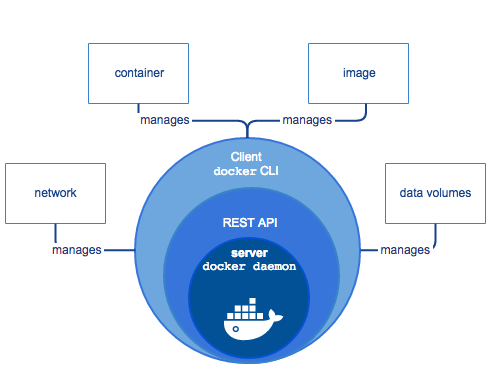
\includegraphics[scale=0.7]{components-flow.png}
	\caption{Конь}
\end{figure}
\clearpage

Docker легковесен и быстр. Он предоставляет устойчивую, рентабельную альтернативу виртуальным машинам на основе гипервизора. Он особенно полезен в условиях высоких нагрузок, например, при создания собственного облака или платформа-как-сервис (platform-as-service). Но он так же полезен для маленьких и средних приложений, когда вам хочется получать больше из имеющихся ресурсов.

Docker состоит из двух главных компонент:

\begin{itemize}
  \item docker: платформа виртуализации с открытым кодом;
  \item docker Hub: наша платформа-как-сервис для распространения и управления docker контейнерами;
\end{itemize}


\subsection{Memcached и Redis}
\label{sec:analysis:mem}

Memcached — программное обеспечение, реализующее сервис кэширования данных в оперативной памяти на основе хеш-таблицы.
С помощью клиентской библиотеки (для C/C++, Ruby, Perl, PHP, Python, Java, .Net и др.) позволяет кэшировать данные в оперативной памяти множества доступных серверов. Распределение реализуется путём сегментирования данных по значению хэша ключа по аналогии с сокетами хэш-таблицы. Клиентская библиотека, используя ключ данных, вычисляет хэш и использует его для выбора соответствующего сервера. Ситуация сбоя сервера трактуется как промах кэша, что позволяет повышать отказоустойчивость комплекса за счет наращивания количества memcached серверов и возможности производить их горячую замену.
В API memcached есть только базовые функции: выбор сервера, установка и разрыв соединения, добавление, удаление, обновление и получение объекта, а также Compare-and-swap. Для каждого объекта устанавливается время жизни, от 1 секунды до бесконечности. При исчерпании памяти более старые объекты автоматически удаляются. Для PHP также есть уже готовые библиотеки PECL для работы с memcached, которые дают дополнительную функциональность.

В первом приближении может показаться, что Redis мало чем отличается от Memcached. И действительно, как Redis, так и Memcached хранят данные в памяти и осуществляют доступ к ним по ключу. Оба написаны на Си и распространяются под лицензией BSD. Но в действительности, между Redis и Memcahced больше различий, чем сходства.

В первую очередь, Redis умеет сохранять данные на диск. Можно настроить Redis так, чтобы данные вообще не сохранялись, сохранялись периодически по принципу copy-on-write, или сохранялись периодически и писались в журнал (binlog). Таким образом, всегда можно добиться требуемого баланса между производительностью и надежностью.

Redis, в отличие от Memcached, позволяет хранить не только строки, но и массивы (которые могут использоваться в качестве очередей или стеков), словари, множества без повторов, большие массивы бит (bitmaps), а также множества, отсортированные по некой величине. Разумеется, можно работать с отдельными элементами списков, словарей и множеств. Как и Memcached, Redis позволяет указать время жизни данных (двумя способами — «удалить тогда-то» и «удалить через …»). По умолчанию все данные хранятся вечно.

Интересная особенность Redis заключается в том, что это — однопоточный сервер. Такое решение сильно упрощает поддержку кода, обеспечивает атомарность операций и позволяет запустить по одному процессу Redis на каждое ядро процессора. Разумеется, каждый процесс будет прослушивать свой порт. Решение нетипичное, но вполне оправданное, так как на выполнение одной операции Redis тратит очень небольшое количество времени (порядка одной стотысячной секунды).
В Redis есть репликация. Репликация с несколькими главными серверами не поддерживается. Каждый подчиненный сервер может выступать в роли главного для других. Репликация в Redis не приводит к блокировкам ни на главном сервере, ни на подчиненных. На репликах разрешена операция записи. Когда главный и подчиненный сервер восстанавливают соединение после разрыва, происходит полная синхронизация (resync).

Также Redis поддерживает транзакции (будут последовательно выполнены либо все операции, либо ни одной) и пакетную обработку команд (выполняем пачку команд, затем получаем пачку результатов). Притом ничто не мешает использовать их совместно.

Еще одна особенность Redis — поддержка механизма publish/subscribe. С его помощью приложения могут создавать каналы, подписываться на них и помещать в каналы сообщения, которые будут получены всеми подписчиками. Что-то вроде IRC-чатика.

\subsection{Jenkins}
\label{sec:analysis:jenkins}

Jenkins – это инструмент непрерывной интеграции, который чаще всего используется для разработки программного обеспечения. Это среда автоматизации, которая выполняет повторяющиеся задания. Jenkins может выполнять и контролировать выполнение команд на удаленных системах, а также всего того, что можно выполнить из командной строки. 

Непрерывная интеграция (continuous integration) — это очень, очень хорошо. Вы настраиваете ее один раз, и все все процессы интеграции происходят без вашего участия. Некоторые плюсы использования Jenkins:
\begin{itemize}
  \item когда кто-то ломает билд, вы узнаете об этом сразу, что позволяет быстро устранить проблему.
  \item вы можете автоматизировать прогон тестов, деплой приложения на тестовый сервер, проверку code style и тому подобные вещи.
  \item также в Jenkins можно хранить собранные deb-пакеты, отчеты о прогоне тестов или Javadoc/Doxygen/EDoc-документацию. 
\end{itemize}
